\newpage
\section{Statyczne badanie właściwości sztucznej skóry}
\label{s_badanie}

Badania właściwości statycznych obejmowały duży zakres prac wykonanych podczas pisania tego dokumentu. Były one podstawą do pogłębiania wiedzy z zakresu działania i zachowania sztucznej skóry oraz posłużyły do budowy prototypu sztucznej skóry umieszczonej później na robocie. 

Badania wykonane przeze mnie były kontynuacją badań prowadzonych przez inż. Macieja Bogusza opisanych w cytowanej przeze mnie pracy. W swoich pracach badał on wiele różnych typów gumy pod kątem przewodności elektrycznej, trwałej odkształcalności oraz pochłanialności energii. Jego badania miały na celu wybór najlepszego materiału nośnego i absorbującego uderzenia, który mógłby posłużyć do budowy sztucznej skóry. Wykonał on także prototyp do~dalszych testów o rozmiarze $4x4$ pola ($25 cm^2$ każde) i~wielkości $40x40 cm$ dwóch fragmentów mikrogumy o grubości $10mm$, każda jako warstwa nośna. Prototyp ten był niego testowany w specjalnie napisanej aplikacji pokazującej napięcie odczytywane na poszczególnych polach czujnika 
\cite{b_report_otrzymane}.

Prowadzone w ramach pracy badania skupiały się na wykonaniu pełnej charakterystyki pojedynczego pola czujnika i ustaleniu równania opisującego zależność pomiędzy przykładanym naciskiem, a odczytywanym napięciem na badanym polu. To badanie jest podstawowym badaniem potrzebnym do obliczeń siły nacisku i umożliwia późniejsze zastosowanie sztucznej skóry w pełni kontrolowany sposób.

Dalsza część badań opierała się na dobraniu zewnętrznych warstw nośnych czujnika, ponieważ wewnętrzne (taśma miedziana i folia Velostat) okazują się działać bardzo dobrze i nie było w nich znacznego pola na poprawę jakości sztucznej skóry. Badania warstw nośnych polegały na doborze odpowiedniej grubości tego samego rodzaju gumy NBR190. Polegały one na pomiarze właściwości gum, pochłanialności energii i rozkładaniu energii przez gumy. Aby poprawnie symulować zachodzące procesy i zapewnić wiarygodne pomiary, badania były przeprowadzane na specjalnie do tego przygotowanych wersjach czujnika. Przygotowane czujniki posiadały tylko jedno pole i pozwalały na~dowolną zamianę górnej i dolnej warstwy nośnej, tak aby przebadać wszystkie możliwe kombinacje budowy czujnika z posiadanych grubości gum. Do badań przygotowane zostały gumy o~grubościach: $5mm$, $10mm$, $15mm$ i $20mm$, z których wycięto pola w~kształcie kwadratu o wymiarach $100x100 mm$. Do każdego z tak przygotowanych pól przyklejono taśmę miedzianą o szerokości $50 mm$. Pomiędzy taśmą miedzianą z dolnej warstwy czujnika i~górnej warstwy czujnika umieszczono docięty na wymiar fragment folii Velostat. Tak~przygotowany czujnik był wykorzystywany w dalszych badaniach.

\subsection{Pomiar zależności masa -- odczyt pojedynczego pola}
\label{ss_badanie_hiperbola}

Pomiar zależności odczytów czujnika w zależności od przyłożonej masy jest pierwszym wykonywanym badaniem, ponieważ jest on kluczowy do wszystkich obliczeń. Bez~znajomości tej zależności surowa wartość odczytana z czujnika nie niesie ze sobą żadnej informacji, jest tylko liczbą. Istotą wyprowadzenia tej zależności jest możliwość wstecznego obliczenia przyłożonego nacisku na podstawie zwracanych danych. Należy także sprawdzić, czy poza naciskiem, wykonane pomiary zależą również od innych zmiennych oraz jaka jest dynamika pracy czujnika.

Do testów charakterystyki pojedynczego pola sztucznej skóry została wykorzystana mniejsza jej wersja używająca tylko jednego pola, aby mieć pewność, że nacisk nie rozkłada się na sąsiadujące elementy. Dodatkowo, czujnik został zbudowany z posiadanych laminatów, które zostały zastosowane jako warstwa nośna zamiast sprężystej gumy. Ewentualne używanie gumy jako materiału nośnego mogłoby zakłócić pomiary przez rozprowadzanie przykładanej siły na boki. Do budowy wnętrza czujnika została wykorzystana taśma miedziana o szerokości $50 mm$ i docięta na odpowiednią wielkość folia Velostat. W efekcie pole efektywne zbudowanego czujnika wynosiło $25 cm^2$. Wykonany czujnik pomiarowy został przedstawiony na rysunku \ref{f_badanie_1_czujnik}.

\begin{figure}[!h]
\centering
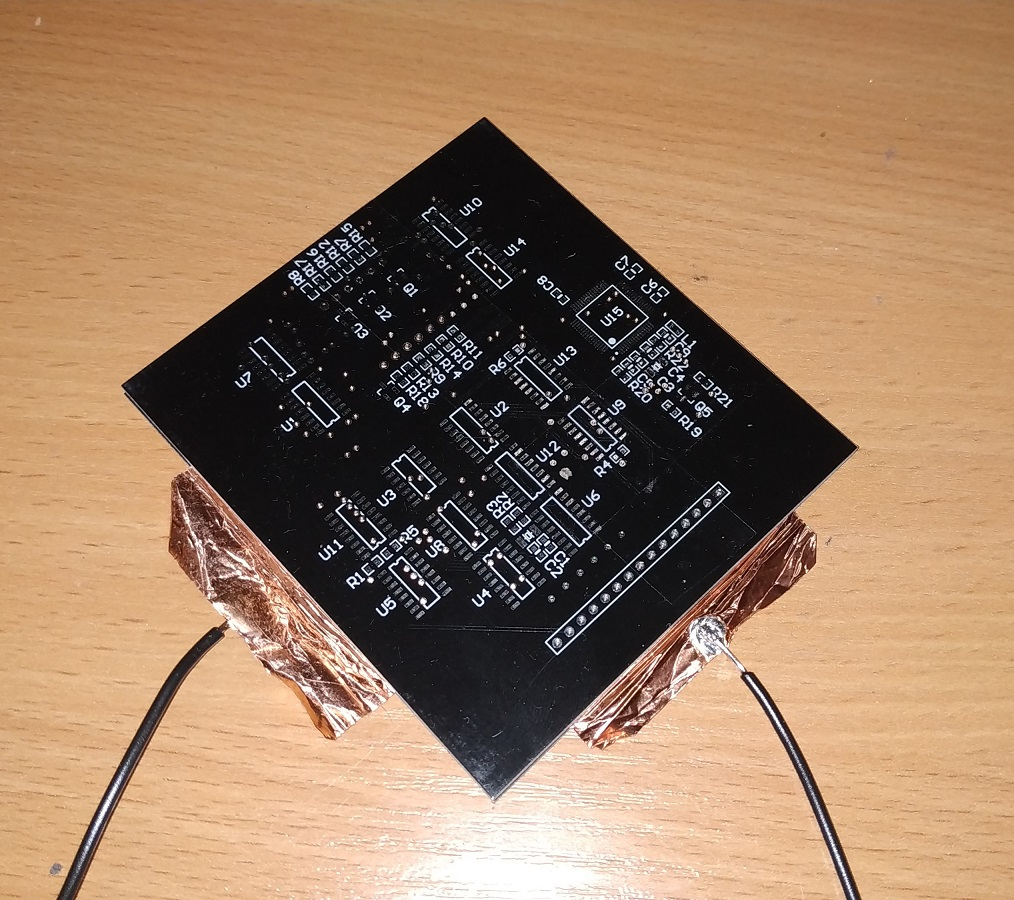
\includegraphics[width=0.5\linewidth]{img/badanie_1_czujnik.jpg}
\caption{Czujnik wykorzystywany do badania charakterystyki folii Velostat}
\label{f_badanie_1_czujnik}
\end{figure}

Wykorzystując zbudowane pole czujnika wyznaczona została charakterystyka jego pracy. Badany był poziom otrzymywanego surowego sygnału w zależności od przykładanego nacisku. Nacisk był wywierany poprzez obciążanie czujnika znaną masą, a surowe pomiary odczytywane w konsoli programu PuTTY.

Pomiary czujnika były zwracane w obszarze $0-3,3V$ co przekłada się na odczyty mikrokontrolera w~zakresie $0-4096$. Taki zakres wynika z wykorzystania wbudowanego w~mikrokontroler STM32F103RB 12-bitowego przetwornika ADC \cite{b_site_F103RB}. Analizując schemat działania czujnika, widoczny na rysunku \ref{f_elektronika_schemat}, możemy zauważyć, że przy braku nacisku (maksymalna rezystancja folii Velostat) otrzymywane są wyniki bliskie maksymalnych możliwych wartości pomiaru ($\sim4000$). Wraz ze zwiększaniem przykładanej siły wartość pomiaru zmniejsza się aż do wartości $\sim1000$. Najniższe uzyskane wartości pomiarów w~okolicy $\sim1000$, a nie $\sim0$ wynikają z użytego układu drabinki Darlingtonowej ULN2803, a~dokładniej z~jej spadku napięcia $V_{CE(sat)}$ wynoszącego w~badanej konfiguracji około $0,75 V$ \cite{b_site_ULN2803}. Pełne wyniki wykonanych pomiarów podczas badań znajdują się w tabeli \ref{t_badanie_1_pomiary}.

\begin{table}[!h]
\centering
\caption{Wykonane pomiary pojedynczego pola czujnika}
\begin{tabular}{|r|r|r|r|r|r|l|}
\hline
\multicolumn{1}{|l|}{Obciążenie {[}g{]}} &
  \multicolumn{1}{l|}{Pomiar 1} &
  \multicolumn{1}{l|}{Pomiar 2} &
  \multicolumn{1}{l|}{Pomiar 3} &
  \multicolumn{1}{l|}{Pomiar 4} &
  \multicolumn{1}{l|}{Pomiar 5} &
  Pomiar 6 \\ \hline
1     & 3930 & 3900 & 3900 & 3870 & 3800 & \multicolumn{1}{r|}{3800} \\ \hline
23    &      &      & 3830 & 3820 &      &                           \\ \hline
51    &      &      & 3800 & 3770 &      &                           \\ \hline
66    &      &      & 3740 & 3720 &      &                           \\ \hline
129   &      &      & 3610 & 3570 &      &                           \\ \hline
324   &      &      & 3300 & 3120 &      &                           \\ \hline
461   &      &      & 3000 & 2850 &      &                           \\ \hline
519   & 3000 & 2900 & 2800 & 2500 & 2600 & \multicolumn{1}{r|}{2500} \\ \hline
1037  & 2400 & 2150 & 2210 & 2030 & 2000 & \multicolumn{1}{r|}{1900} \\ \hline
1555  & 1910 & 1840 & 1670 & 1580 & 1530 & \multicolumn{1}{r|}{1540} \\ \hline
2073  & 1670 & 1610 & 1470 & 1380 & 1340 & \multicolumn{1}{r|}{1380} \\ \hline
2591  & 1560 & 1480 & 1300 & 1265 & 1180 & \multicolumn{1}{r|}{1210} \\ \hline
3109  & 1390 & 1340 & 1220 & 1200 & 1130 & \multicolumn{1}{r|}{1130} \\ \hline
3642  & 1290 & 1270 & 1140 & 1111 &      &                           \\ \hline
4175  & 1220 & 1240 & 1100 & 1090 &      &                           \\ \hline
4708  & 1170 &      &      &      &      &                           \\ \hline
5248  & 1140 &      &      &      &      &                           \\ \hline
78000 & 890  &      &      &      &      &                           \\ \hline
\end{tabular}
\label{t_badanie_1_pomiary}
\end{table}

Wyznaczanie charakterystyki polegało na kolejnym obciążaniu czujnika przedmiotami o znanej masie. Czujnik miał bardzo niezadowalającą dynamikę i~ciężko było wyznaczyć jednoznaczną charakterystykę czujnika. Dynamika czujnika objawiała się głównie na~gwałtownym osiągnięciu wartości w okolicy wartości końcowej i późniejszym powolnym dochodzeniu do tej wartości. Osiąganie wartości końcowej czasami zajmowało nawet kilka minut. Ze względu na wykorzystanie czujnika w dość dynamicznym środowisku, które musi szybko reagować na bodźce, nie jest to pożądana charakterystyka. Na~szczęście, czujnik ten też natychmiastowo (w kontekście częstotliwości wykonywanych pomiarów) osiąga wartość w okolicach docelowej. Można ten fakt wykorzystać i~ustalić charakterystykę czujnika w pierwszej fazie po otrzymaniu bodźca.

Układ sprawiał też dziwne wrażenie, jakby z upływam czasu zmieniał swoje odczyty, co jest również widoczne w tabeli \ref{t_badanie_1_pomiary}. Pomiary 1, 2, 3 i 4 wykonane zostały jednego dnia. Pomiary 1 i 2 były prowadzone równolegle - naprzemiennie prowadzono pomiary wartości dla danego obciążenia z chwilowym odpuszczaniem, aby rozluźnić naprężenia czujnika pomiędzy pomiarami. Później, tego samego dnia, wykonane zostały pomiary 3 i 4, mające na celu sprawdzenie szybkości reakcji i wartości końcowej przy danym obciążeniu. Pomiar 3 był wykonywany od razu w chwili położenia obciążenia, pomiar 4 został zmierzony na tym samym przedmiocie bez zmian obciążenia w momencie ustabilizowania się odczytów. Pomiary 5 i 6 zostały wykonane kilka dni później, jako pomiary uzupełniające, mające pokazać poprawność i stałość poprzednich pomiarów. 

Nie wszystkie z wykonanych pomiarów zostały wykonane na pełnym zakresie testowym. Brak pomiarów wartości dla niskich obciążeń spowodowany był początkowym brakiem przykładania większej uwagi dla nacisku w tym zakresie, ponieważ nie spodziewano się wywierania tak lekkiego nacisku na powierzchnię robota. 
Pomiar obciążeniem $78000 g$ został wykonany poprzez stanięcie człowieka na czujniku i miał za zadanie ustalić pomiar czujnika przy teoretycznie nieskończonym obciążeniu. Obciążenie $1 g$ dostało umownie przypisane dla braku dodatkowego obciążenia.

Za rozbieżności podczas wykonywania pomiarów odpowiedzialne może być kilka czynników, w tym zmęczenie materiału folii, wpływ temperatury (której nie mierzono dokonując pomiar) i niestała charakterystyka drabinki Darlingtonowej (która też może zmieniać się w zależności od temperatury \cite{b_site_ULN2803}).

% \begin{figure} [!h]
%   \begin{subfigure}[b]{0.5\linewidth}
%     \centering
%     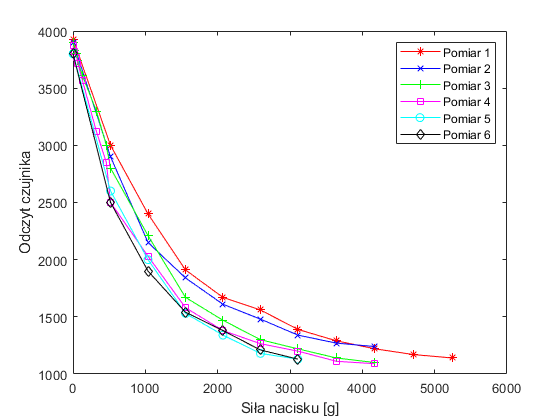
\includegraphics[width=1\linewidth]{img/badanie_1_pomiar.png} 
%     \caption{Pomiary w skali standardowej} 
%   \end{subfigure}%% 
%   \begin{subfigure}[b]{0.5\linewidth}
%     \centering
%     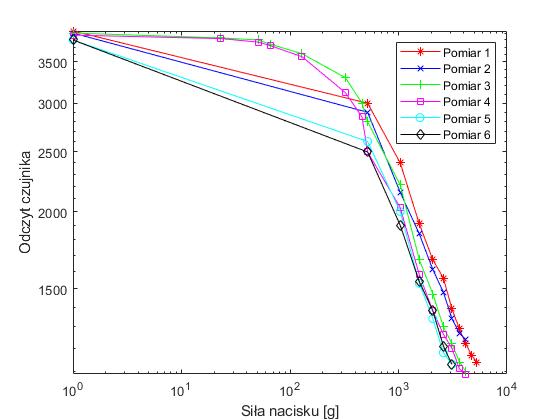
\includegraphics[width=1\linewidth]{img/badanie_1_logarytm.png}
%     \caption{Pomiary w skali logarytmicznej}
%   \end{subfigure} 
%   \centering
%   \caption{Wykonane pomiary pojedynczego pola}
%   \label{f_badanie_1_pomiar} 
% \end{figure}

Pełne wykresy zebranych danych przedstawiono na wykresie \ref{f_badanie_1_standard}, zostały one również przedstawione w skali logarytmicznej na wykresie \ref{f_badanie_1_logarytm}. Wykres z logarytmiczną skalą został wykonany, ponieważ pierwsze spojrzenie na otrzymane pomiary sugerowało charakterystykę logarytmiczną czujnika. Założenie to po przeanalizowaniu wykresu w~skali logarytmicznej okazało się nieprawdziwe.

\begin{figure}[!h]
    \centering 
    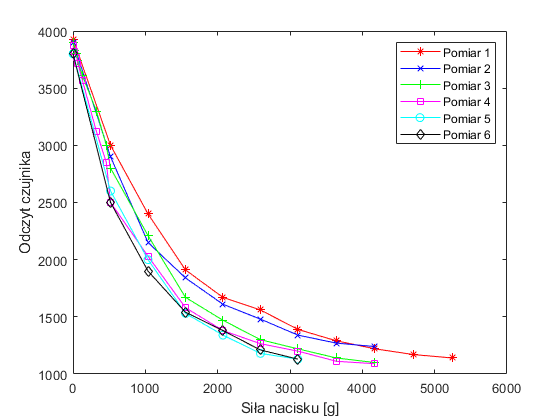
\includegraphics[width=0.85\linewidth]{img/badanie_1_pomiar.png}
    \caption{Wykonane pomiary pojedynczego pola -- skala liniowa}
    \label{f_badanie_1_standard}
\end{figure}

\begin{figure}[!h]
    \centering 
    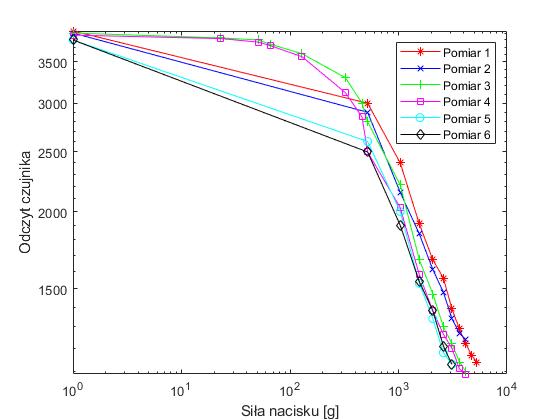
\includegraphics[width=0.85\linewidth]{img/badanie_1_logarytm.png}
    \caption{Wykonane pomiary pojedynczego pola -- skala logarytmiczna}
    \label{f_badanie_1_logarytm}
\end{figure}

Jak można zauważyć, wykonane odczyty układają się w dodatnią część wykresu hiperboli i ten kształt przyjęto w procesie aproksymacji. Standardowe równanie hiperboli ma postać:
\begin{equation}
    f(x) = y + \frac{a}{(x-x_0)}
\end{equation}
gdzie parametry $y$, $a$ i $x_0$ muszą zostać dobrane indywidualnie do naszego przypadku. Parametr $y$ odpowiada za przesunięcie wykresu hiperboli w osi pionowej, $x_0$ za przesunięcie w osi poziomej, natomiast $a$ odpowiada za sam kształt hiperboli.

W celu przyspieszenia wyznaczenia parametrów hiperboli użyty został program Matlab i jego funkcja wbudowana \textit{fminunc}. Funkcja ta jest w stanie znaleźć minimum zadanej funkcji wielu zmiennych używając wybranego algorytmu (Quasi-Newtonowski lub regionu zaufania). Algorytm optymalizacji przyjmuje jako parametr funkcję do optymalizacji (w~analizowanym przypadku - hiperbola), punkt początkowy poszukiwania rozwiązania oraz parametry wpływające na wewnętrzne działanie algorytmu m.in. algorytm działania czy ilość wypisywanych informacji w trakcie obliczeń \cite{b_site_Matlab_fminunc}.

Ważną sprawą podczas używania tego sposobu minimalizacji jest zwracanie przez algorytm minimum lokalnego, co oznacza, że zwrócone rozwiązanie nie musi być najlepsze ze wszystkich istniejących \cite{b_site_Matlab_fminunc}. Dlatego, aby zwiększyć prawdopodobieństwo znalezienia najlepszego rozwiązania, algorytm został uruchomiony wielokrotnie z różnymi, losowymi punktami początkowymi. Jako najlepsze rozwiązanie wybrane zostało to, które zwróciło najmniejszy błąd aproksymacji. Błąd aproksymacji, tak samo jak parametr minimalizacji, został określony jako norma Euklidesowa wszystkich punktów. Równanie normy Euklidesowej opisane jest wzorem:
\begin{equation}
    e = \sqrt{\sum_{i=1}^{n} (f(x_i) - y_i)^2}
\end{equation}
gdzie $e$ jest obliczonym błędem aproksymacji.

Sama aproksymacja została wykonana tylko w oparciu o dane z 3 pomiaru, ponieważ najlepiej oddają one charakterystykę pracy sensora i są pełne - zawierają dane również dla pomiarów z niskim obciążeniem czujnika. Dodatkowo, były one zbierane w~momencie nałożenia obciążenia na czujnik, co jest pożądane w~projektowanej aplikacji i najlepiej odzwierciedla faktyczne środowisko, w~którym czujnik będzie pracować. 

Po wstępnym wykonaniu aproksymacji za pomocą Matlaba zauważono pewne niedoskonałości dopasowanej hiperboli. Mimo otrzymania niskiego błędu aproksymacji hiperbola wydaje się być zbyt mocno przystosowana do danych przy niskiej sile nacisku, gdzie pomiary są gęstsze, a gorzej przystosowana w dalszej części wykresu. Ponadto, wykres z automatycznie dobieranymi parametrami poza badanym zakresem ($>5 kg$) wciąż zdaje się dążyć w dół, mimo iż z tendencji wykresu wynika inaczej. Dlatego postanowiono ręcznie dobrać parametry hiperboli bazując na tych otrzymanych automatycznie. Głównym celem dopasowania było zmniejszenie współczynnika hiperboli i podniesienie wykresu przy dużym nacisku (zwiększenie $y$). Tak dobrane parametry lepiej oddają zachowanie czujnika, mimo iż prezentują większą obliczoną wartość błędu.

Otrzymane podczas obu aproksymacji parametry zostały przedstawione w tabeli \ref{t_badanie_1_aproksymacja}, a~wykres wraz z danymi służącymi do aproksymacji jest przedstawiony na wykresie \ref{f_badanie_1_aproksymacja}.

\begin{figure}[!h]
    \centering 
    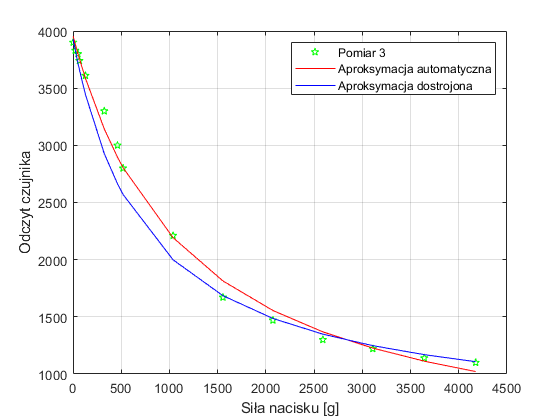
\includegraphics[width=0.85\linewidth]{img/badanie_1_aproksymacja.png}
    \caption{Aproksymacja wykonanych pomiarów hiperbolą}
    \label{f_badanie_1_aproksymacja}
\end{figure}

\begin{table}[!h]
\centering
\caption{Wyniki aproksymacji pomiarów pola czujnika}
\begin{tabular}{|l|r|r|r|r|}
\hline
Sposób aproksymacji       & \multicolumn{1}{c|}{$y$} & \multicolumn{1}{c|}{$a$} & \multicolumn{1}{c|}{$x_0$} & \multicolumn{1}{l|}{Błąd aproksymacji} \\ \hline
Automatyczna aproksymacja & 196                    & 4409590                & 1172                   & 286,4597                               \\ \hline
Ręczna aproksymacja       & 600                    & 2500000                & 750                    & 627,271                                \\ \hline
\end{tabular}
\label{t_badanie_1_aproksymacja}
\end{table}

\subsection{Pomiar podstawowych parametrów materiału nośnego}

Od tego momentu rozpoczęto wykonywać pomiary już bezpośrednio na materiale nośnym, a dokładniej złożeniu dwóch materiałów nośnych symulujących zbudowany gotowy czujnik. Do wykonania pomiarów opisanych w tym podrozdziale nie było konieczności budować specjalnego stanowiska pomiarowego. Były to pomiary podstawowych wartości, które można wykonać bez sprzętu laboratoryjnego. Pomiary te obejmowały:
\begin{itemize}
    \item masę czujnika,
    \item grubość czujnika,
    \item minimalny promień zgięcia materiału.
\end{itemize}

Jak można zauważyć, parametry te nie są kluczowe w wybranym zastosowaniu, ale mają kluczowe znaczenie, jeśli czujnik miałby być w przyszłości wykorzystywany na robotach posiadających dużą powierzchnię i~cała ta powierzchnia miałaby być pokryta sztuczną skórą. Wtedy wymienione wyżej parametry nabierają znaczenia, ponieważ wartości te odgrywają spore znaczenie w działaniu robota. Zwiększona masa ma negatywny wpływ na prędkość poruszania się robota oraz pobór energii potrzebnej do poruszania się, co~może skutkować np. znacznie krótszym czasie pracy na baterii. Większa masa sztucznej skóry utrudnia również zamocowanie jej na robocie i~wymaga do tego solidniejszych, bardziej skomplikowanych rozwiązań. Natomiast większa grubość czujnika powoduje, że robot zajmuje więcej przestrzeni, co może powodować większe prawdopodobieństwo wchodzenia w kolizje.

Jako pierwszy wykonany został pomiar grubości, który tak właściwie nie musiał być wykonywany, ponieważ posiadane próbki gumy miały grubość ustaloną przez producenta. 
Grubości warstwy taśmy miedzianej wynoszące $25\mu m$ \cite{b_site_kamami_tasma} każda oraz grubość folii Velostat wynosząca $0,1 mm$ \cite{b_site_kamami_folia} przy grubości dwóch warstw gumy wynoszącej w~najmniejszym przypadku $10 mm$ była znikoma. 
Przy grubości dwóch warstw gumy, wynoszącej w najmniejszym przypadku $10mm$, grubości warstw taśmy miedzianej wynoszące $25um$ każda \cite{b_site_kamami_tasma} oraz grubość folii Velostat wynosząca $0,1mm$ \cite{b_site_kamami_folia} były znikome.
Dokładna względna różnica grubości przy doliczeniu miedzi i folii Velostat wynosiła w tym przypadku $1,5\%$ i jest to największa możliwa do~osiągnięcia niedokładność. Z tego powodu pomiary grubości zostały wykonane poprzez dodanie grubości gum składających się na budowę danego czujnika.

Kolejną podstawową wartością łatwą do zmierzenia jest masa materiałów nośnych. Cały proces wymaga jedynie działającej wagi, kładzeniu na niej gotowych czujników i~odczycie pomiarów. Taka procedura została również wykonana w tym przypadku, podczas wykonywania tego pomiaru. Do pomiaru masy posłużyła ustawiona na równym podłożu waga kuchenna o zakresie pomiarowym $0-5000 g$ i dokładności $\pm 1g$. Wykorzystane stanowisko pomiarowe zostało przedstawione na rysunku \ref{f_badanie_2_stanowisko_waga}.

\begin{figure}[!h]
    \centering 
    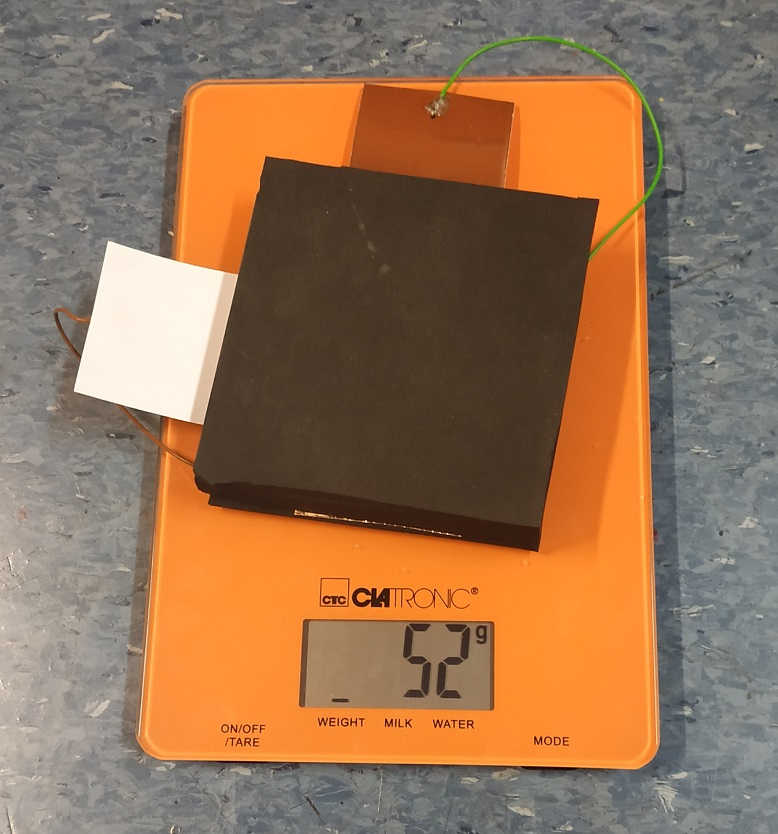
\includegraphics[width=0.5\linewidth]{img/badanie_2_stanowisko.jpg}
    \caption{Stanowisko pomiarowe do badania masy sztucznej skóry}
    \label{f_badanie_2_stanowisko_waga}
\end{figure}

Uzyskanie wartości wagi jest jeszcze możliwe na inny sposób - poprzez wyliczenie masy znając zajmowaną objętość czujnika oraz gęstość materiału użytego do jego budowy. Znając gęstość gumy NBR190, wynoszącą $190 \frac{kg}{m^3}$ oraz grubości poszczególnych warstw można skorzystać z przekształconego wzoru na gęstość:
\begin{equation}
    m = \rho*V
\end{equation}
Z tego wzoru można obliczyć masę użytego materiału nośnego, gdzie $m$ jest masą, $\rho$ gęstością, a $V$ objętością czujnika.

Zarówno wyniki pomiarów przy użyciu wagi, jak i obliczonych wartości zostały przedstawione w tabeli \ref{t_badanie_2_wyniki}. Widoczne różnice pomiędzy masą zmierzoną, a obliczoną są niewielkie i zazwyczaj wyższe wartości osiągają wartości zmierzone. Rozbieżności te mogą wynikać z niedokładnie przygotowanych pól czujnika oraz dodatkowo umieszczonych na gumie pasów folii miedzianej i okablowania zwiększających ich masę. Ponadto, w moim odczuciu waga kuchenna nie jest urządzeniem, w którym deklarowana przez producenta dokładność jest utrzymana w trakcie pomiaru i wyniki pomiarów otrzymane w ten sposób mają przez to większe niedokładności.

\begin{table}[!h]
\centering
\caption{Pomiar wagi testowanych materiałów nośnych}
\begin{tabular}{r|r|c|c}
\multicolumn{1}{l|}{\begin{tabular}[c]{@{}l@{}}Grubość górnej\\ warstwy {[}mm{]}\end{tabular}} & \multicolumn{1}{l|}{\begin{tabular}[c]{@{}l@{}}Grubość dolnej\\ warstwy {[}mm{]}\end{tabular}} & \multicolumn{1}{l|}{\begin{tabular}[c]{@{}l@{}}Waga zmierzona\\ {[}g{]}\end{tabular}} & \multicolumn{1}{l}{\begin{tabular}[c]{@{}l@{}}Waga obliczona\\ {[}g{]}\end{tabular}} \\
\hline
\hline
5                                                                                             & 5                                                                                             & 22                                                                                   & 19                                                                                   \\
5                                                                                             & 10                                                                                            & 33                                                                                   & 28,5                                                                                 \\
5                                                                                             & 15                                                                                            & 40                                                                                   & 38                                                                                   \\
5                                                                                             & 20                                                                                            & 52                                                                                   & 47,5                                                                                 \\
\hline
10                                                                                            & 5                                                                                             & 33                                                                                   & 28,5                                                                                 \\
10                                                                                            & 10                                                                                            & 45                                                                                   & 38                                                                                   \\
10                                                                                            & 15                                                                                            & 50                                                                                   & 47,5                                                                                 \\
10                                                                                            & 20                                                                                            & 61                                                                                   & 57                                                                                   \\
\hline
15                                                                                            & 5                                                                                             & 40                                                                                   & 38                                                                                   \\
15                                                                                            & 10                                                                                            & 50                                                                                   & 47,5                                                                                 \\
15                                                                                            & 15                                                                                            & 53                                                                                   & 57                                                                                   \\
15                                                                                            & 20                                                                                            & 65                                                                                   & 66,5                                                                                 \\
\hline
20                                                                                            & 5                                                                                             & 52                                                                                   & 47,5                                                                                 \\
20                                                                                            & 10                                                                                            & 61                                                                                   & 57                                                                                   \\
20                                                                                            & 15                                                                                            & 65                                                                                   & 66,5                                                                                 \\
20                                                                                            & 20                                                                                            & 77                                                                                   & 76                                                                                  
\end{tabular}
\label{t_badanie_2_wyniki}
\end{table}

Same wyniki są natomiast zgodnie z przewidywaniami mocno liniowe, a waga czujnika rośnie proporcjonalnie do grubości użytego czujnika. Pozwala to stwierdzić, że pod względem samej masy najlepszy jest najcieńszy czujnik.

Ostatnim z wykonanych pomiarów jest pomiar minimalnego promienia zgięcia. Minimalny promień zgięcia materiału jest najmniejszym promieniem łuku, który może przyjąć materiał bez jego przełamania, uszkodzenia lub zmniejszenia jego trwałości w sposób trwały lub na czas zgięcia. Przy zastosowaniu gumy jako warstwy nośnej sztucznej skóry ważne jest, aby wybrany materiał był w stanie jak najmocniej się zginać, by mógł on dopasować się do kształtu robota, a w szczególności jego rogów. W badanym przypadku nie jest to jednak krytyczne kryterium. Robot, na którym zostanie założona sztuczna skóra ma promienie gięcia obudowy równe $\sim 10mm$, co jest stosunkowo dużym promieniem. Sam czujnik nie zostanie jednak założony bezpośrednio na obudowę, tylko na specjalny szkielet, który nie będzie posiadał krzywizn o bardzo małym promieniu.

Wstępny pomiar minimalnego promienia gięcia wykonywany dłońmi wykazał jednak, że wszystkie wybrane do badań materiały pozwalają na ich zginanie na praktycznie zerowym promieniu bez widocznej utraty swoich właściwości. Powodem tego jest badanie gumy, która strukturalnie jest bardzo elastyczna.
Widoczna była jedynie różnica w sile potrzebnej, aby dany materiał doprowadzić do zgięcia z tak niewielkim promieniem. Dlatego wykonane pomiary nie opierały się ostatecznie na wykryciu minimalnego promienia zgięcia materiału, lecz na pomiarze siły potrzebnej do doprowadzenia materiału do tego samego promienia zgięcia.

Pomiary te zostały wykonane na stanowisku, gdzie fragment gumy został stabilnie zamocowany w imadle.
Pomiar siły potrzebnej do~osiągnięcia tej pozycji był wykonywany za pomocą siłomierza z zakresem pomiaru $0-100 N$ i dokładności $\pm 2 N$. 
Pomiar był wykonywany poprzez ściąganie gumy za pomocą siłomierza w dół, aż do momentu, kiedy guma owinęła się na konstrukcji imadła dotykając jego zewnętrznej części. W~tym momencie pobierany był pomiar siły.
Podczas pomiarów czasami miedziana taśma pękała, dlatego też większość pomiarów została wykonana na gumie bez naklejonej taśmy miedzianej, która nie ma żadnego wpływu na wynik tego pomiaru.
Stanowisko pomiarowe podczas wykonywania pomiaru zostało przedstawione na rysunku \ref{f_badanie_2_giecie}, a wyniki pomiarów w tabeli \ref{t_badanie_2_giecie}. 

\begin{table}[!h]
\centering
\caption{Pomiar siły potrzebnej do zgięcia gumy}
\begin{tabular}{r|c}
Grubość gumy {[}mm{]} & Zmierzona siła {[}N{]} \\
\hline
\hline
5                     & 2                      \\
\hline
10                    & 10                     \\
\hline
15                    & 24                     \\
\hline
20                    & 42                    
\end{tabular}
\label{t_badanie_2_giecie}
\end{table}

\begin{figure}[!h]
    \centering 
    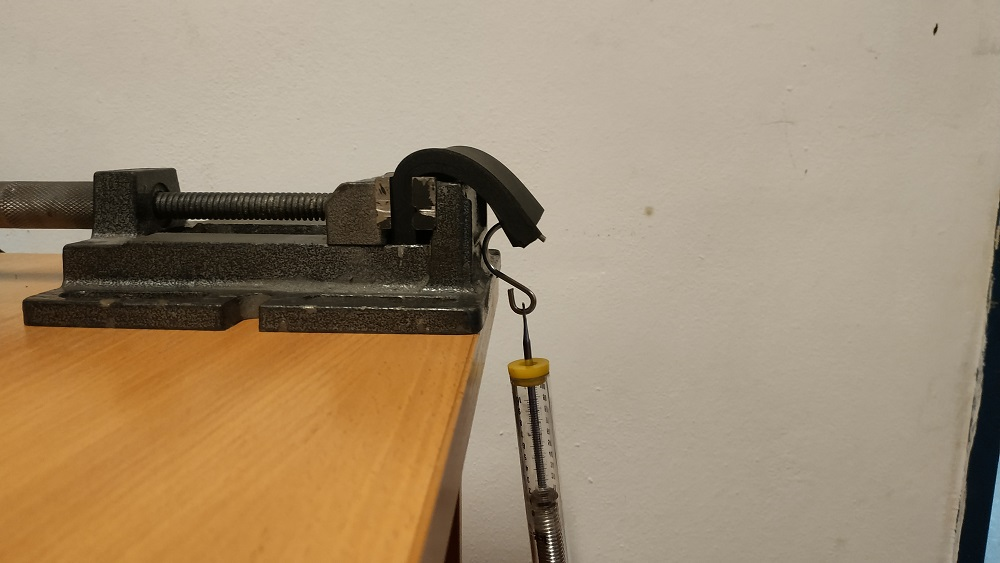
\includegraphics[width=0.9\linewidth]{img/badanie_gietkosc.jpg}
    \caption{Stanowisko pomiarowe siły wymaganej do zgięcia gumy}
    \label{f_badanie_2_giecie}
\end{figure}



Jak można zauważyć, chudsze warstwy gumy potrzebują użycia znacznie mniejszej siły do uzyskania wymaganego promienia zgięcia. Mimo iż potencjalnie każdy z materiałów nadaje się do użycia to te, które łatwiej się zginają są preferowane. Mniejsza siła potrzebna do zgięcia materiału umożliwia wykorzystanie do utrzymania jej w wymaganym kształcie lżejszych materiałów mocujących. Wykorzystanie dwustronnej taśmy klejącej jest prostszym i szybszym rozwiązaniem niż np. śrub, mimo iż taśma klejąca nie posiada tak samo dużej siły trzymania co śruby. Z tego powodu w tym teście również najlepsze do zastosowania okazują się być najcieńsze gumy.

Po analizie wyników można stwierdzić, że parametry mechaniczne jednoznacznie wskazują na to, że najlepszymi materiałami do wykorzystania są najcieńsze gumy. Posiadają one zarówno najmniejszą masę, najmniejszą grubość, jak i nie potrzeba wielkiej siły, aby doprowadzić je do zgięcia w~wymagany kształt.

\subsection{Badanie pochłanialności energii materiału nośnego}

Pochłanialność energii jest ważną cechą skóry. Odpowiada ona za znaczne zmniejszenie uszkodzeń zarówno robota, jak i otoczenia w wyniku uderzeń. Naturalnym jest, że~skóra powinna tłumić jak największą część energii otrzymywanego uderzenia.

Pomiar pochłanialności energii wykonany został przez upuszczanie na kolejne badane konfiguracje czujnika standardowej piłeczki golfowej, a następnie pomiar wysokości na jaką się ona odbijała. Wykorzystane do tego celu stanowisko pomiarowe zostało przedstawione na rysunku \ref{f_badanie_3_stanowisko}. Na rysunku \ref{f_badanie_3_stanowisko} widoczna jest przede wszystkim plansza z podziałką do~odczytu wysokości, na którą odbiła się upuszczana piłeczka. Plansza ta pozwalała na dokładny odczyt wartości z dokładnością do $\pm 5mm$, a pomiary o większej dokładności były szacowane (pozwalała na to jakość użytej kamery).

\begin{figure}[!h]
    \centering 
    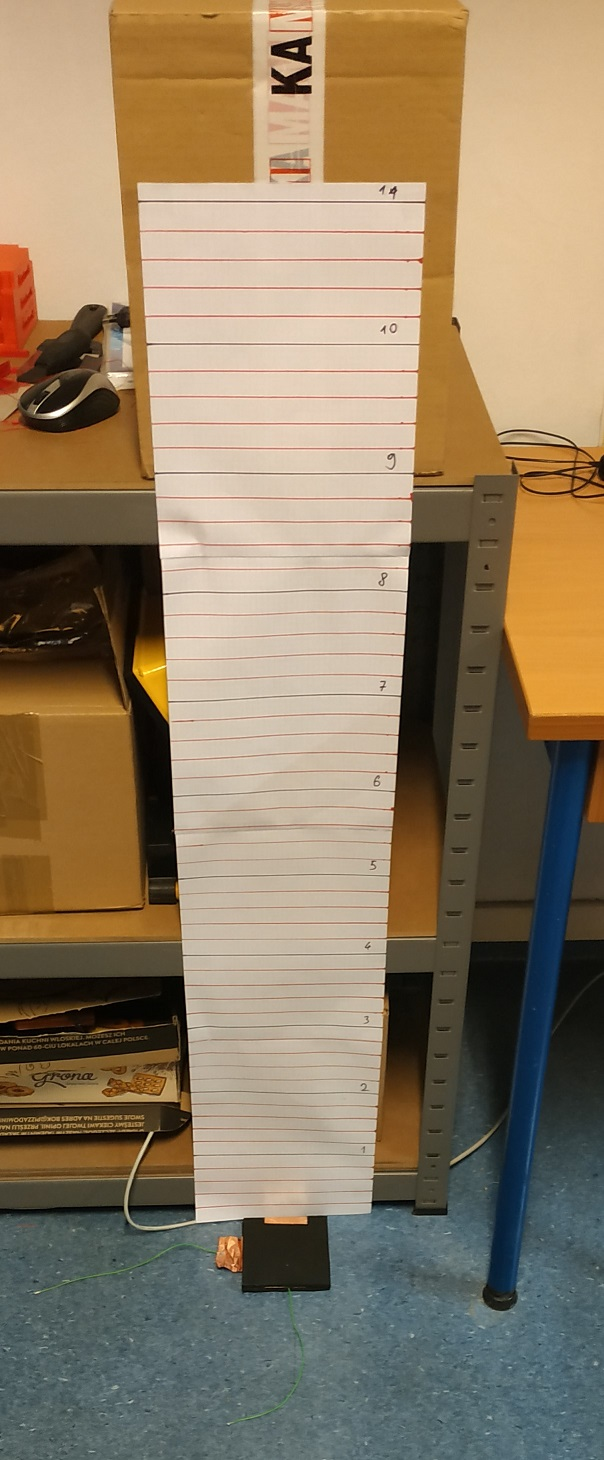
\includegraphics[width=0.3\linewidth]{img/badanie_3_stanowisko.jpg}
    \caption{Stanowisko pomiarowe do badania pochłanialności energii}
    \label{f_badanie_3_stanowisko}
\end{figure}

Aby móc dokładnie odczytywać wysokość, na którą odbiła się piłeczka golfowa została użyta szybka kamera, nagrywająca obraz w $100$ klatkach na sekundę w rozdzielczości $1280x720 px$. Odtworzenie nagranych testów pozwoliło poklatkowo bardzo dokładnie odczytać wysokość, na jaką wzniosła się piłeczka po odbiciu od badanego czujnika. Kamera była umieszczona w odległości $2000 mm$ od planszy, a~pomiary były dokonywane w~odległości $\sim 50 mm$ od planszy. W ten sposób zminimalizowano wpływ występującego przesunięcia kątowego i~upewniono się, że odczytane z obrazu wartości wysokości odbicia są jak najmniej zniekształcone. Oprócz pominięcia błędu kątowego pominięto również istniejące opory, w tym opór powietrza.

Piłeczka golfowa była zrzucana na czujnik z wysokości dokładnie $1000 mm$ nad powierzchnią czujnika. Oznacza to, że wysokość upuszczania piłeczki zmieniała się w~zależności od tego, jak gruby czujnik był badany. Pozwoliło to na otrzymanie danych, które~można porównywać pomiędzy czujnikami tylko poprzez odjęcie grubości czujnika od wysokości odbicia. Dlatego też wszystkie zaprezentowane w tej pracy wyniki uwzględniają wykonanie tego prostego obliczenia i zostały opisane jako względne - uwzględniając wysokość badanego czujnika. Każdy z wykonanych pomiarów został powtórzony przynajmniej 3 razy, a~uzyskany wynik - uśredniony.

Zanim przystąpiono do właściwych pomiarów wykonany został także pomiar tego, jaką część energii pochłania podłoże, na którym testowane były czujniki, aby uzyskać względną wartość o jaką tłumią zbudowane czujniki. Pomiar ten wykonany został analogicznie do opisanej powyżej metody, poprzez kilkukrotne upuszczenie piłeczki i obliczenie średniej wysokości odbicia. Otrzymano w ten sposób wartość $808,33 mm$ jako średnią wysokość odbicia, co przekłada się na pochłanialność energii równą $19,17 \%$. Wyniki procentowej pochłanialności energii testowanych czujników przyrównywane są do pomiarów pochłanialności podłoża właśnie, a nie do wysokości upuszczania piłeczki. Całość otrzymanych wyników przeprowadzonych badań widoczna jest w tabeli \ref{t_badanie_3_wyniki_2}. Największe uzyskane wartości pochłanialności zostały oznaczone kolorem zielonym, a najgorsze kolorem czerwonym. Wyniki rozciągające się pomiędzy tymi skrajnościami zostały oznaczone odpowiednio przechodzącymi przez barwę pomarańczową kolorami.

\begin{table}
\centering
\footnotesize
\caption{Wyniki pomiarów pochłanialności energii użytych gum}
\label{t_badanie_3_wyniki_2}
\begin{tabular}{|l|c|c|c|c|c|c|c|c|}
\hline
\begin{tabular}[c]{@{}l@{}}Grubość\\ dolnej\\ warstwy\\ {[}mm{]}\end{tabular} &
  \multicolumn{4}{l|}{5} &
  \multicolumn{4}{l|}{10} \\ \hline
\begin{tabular}[c]{@{}l@{}}Grubość\\ górnej\\ warstwy\\ {[}mm{]}\end{tabular} &
  \multicolumn{1}{l|}{5} &
  \multicolumn{1}{l|}{10} &
  \multicolumn{1}{l|}{15} &
  \multicolumn{1}{l|}{20} &
  \multicolumn{1}{l|}{5} &
  \multicolumn{1}{l|}{10} &
  \multicolumn{1}{l|}{15} &
  \multicolumn{1}{l|}{20} \\ \hline
 &
  80 &
  75 &
  98 &
  97 &
  65 &
  70 &
  85 &
  85  \\ \cline{2-9} 
 &
  72 &
  80 &
  101 &
  77 &
  72 &
  72 &
  87 &
  90 \\ \cline{2-9} 
 &
  75 &
  75 &
  102 &
  101 &
  75 &
  78 &
  87 &
  86 \\ \cline{2-9} 
 &
  77 &
  80 &
   &
  95 &
  73 &
  76 &
   &
  88 \\ \cline{2-9} 
 &
  82 &
  85 &
   &
  110 &
  72 &
   &
   &
   \\ \cline{2-9} 
\multirow{-6}{*}{\begin{tabular}[c]{@{}l@{}}Pomiary\\ względne\\ wysokości\\ odbicia\\ {[}mm{]}\end{tabular}} &
  90 &
  84 &
   &
  100 &
  82 &
   &
   &
   \\ \hline
\begin{tabular}[c]{@{}l@{}}Średnia\\ względna\\ wysokość\\ odbicia\end{tabular} &
  79,33 &
  79,83 &
  100,33 &
  96,67 &
  73,17 &
  74,00 &
  86,33 &
  87,25  \\ \hline
\begin{tabular}[c]{@{}l@{}}Pochłanialność\\ energii {[}\%{]}\end{tabular} &
  \cellcolor[HTML]{68EE2A}90,19 &
  \cellcolor[HTML]{70ED2D}90,12 &
  \cellcolor[HTML]{FF0803}87,59 &
  \cellcolor[HTML]{FF4721}88,04 &
  \cellcolor[HTML]{00FF00}90,95 &
  \cellcolor[HTML]{0EFC06}90,85 &
  \cellcolor[HTML]{DDDB59}89,32 &
  \cellcolor[HTML]{EDD95F}89,21 \\ \hline
\end{tabular}
\end{table}

\addtocounter{table}{-1}
\begin{table}
\centering
\footnotesize
\captionsetup{list=no}
\caption{ \textbf{(c.d.)} Wyniki pomiarów pochłanialności energii użytych gum}
\begin{tabular}{|l|c|c|c|c|c|c|c|c|}
\hline
\begin{tabular}[c]{@{}l@{}}Grubość\\ dolnej\\ warstwy\\ {[}mm{]}\end{tabular} &
  \multicolumn{4}{l|}{15} &
  \multicolumn{4}{l|}{20} \\ \hline
\begin{tabular}[c]{@{}l@{}}Grubość\\ górnej\\ warstwy\\ {[}mm{]}\end{tabular} &
  \multicolumn{1}{l|}{5} &
  \multicolumn{1}{l|}{10} &
  \multicolumn{1}{l|}{15} &
  \multicolumn{1}{l|}{20} &
  \multicolumn{1}{l|}{5} &
  \multicolumn{1}{l|}{10} &
  \multicolumn{1}{l|}{15} &
  \multicolumn{1}{l|}{20} \\ \hline
   &
  77 &
  83 &
  91 &
  94 &
  98 &
  91 &
  91 &
  98 \\ \cline{2-9} 
 &
  85 &
  90 &
  97 &
  89 &
  100 &
  89 &
  107 &
  99 \\ \cline{2-9} 
 &
  85 &
  78 &
  95 &
  99 &
  100 &
  94 &
  85 &
  101 \\ \cline{2-9} 
  &
  87 &
   &
  91 &
  86 &
  98 &
  84 &
  115 &
  100 \\ \cline{2-9} 
 &
   &
   &
   &
  95 &
  103 &
   &
  106 &
  101 \\ \cline{2-9} 
\multirow{-6}{*}{\begin{tabular}[c]{@{}l@{}}Pomiary\\ względne\\ wysokości\\ odbicia\\ {[}mm{]}\end{tabular}} &
    &
   &
   &
   &
  85 &
   &
   &
   \\ \hline
   \begin{tabular}[c]{@{}l@{}}Średnia\\ względna\\ wysokość\\ odbicia\end{tabular} &
  83,50 &
  83,67 &
  93,50 &
  92,60 &
  97,33 &
  89,50 &
  100,80 &
  99,80 \\ \hline
\begin{tabular}[c]{@{}l@{}}Pochłanialność\\ energii {[}\%{]}\end{tabular} &
  \cellcolor[HTML]{AEE346}89,67 &
  \cellcolor[HTML]{B1E247}89,65 &
  \cellcolor[HTML]{FF7D3B}88,43 &
  \cellcolor[HTML]{FF8D43}88,54 &
  \cellcolor[HTML]{FF3B1C}87,96 &
  \cellcolor[HTML]{FFC25C}88,93 &
  \cellcolor[HTML]{FF0000}87,53 &
  \cellcolor[HTML]{FF1108}87,65 \\ \hline
\end{tabular}
\end{table}

Po przeanalizowaniu danych można zauważyć, że wykorzystane czujniki niezależnie od użytych grubości gum dają podobne wartości wysokości odbicia. Wartości te mieszczą się w przedziale $73,17-100,80mm$. Pomimo tak podobnych wyników widoczne są również wyraźnie różnice pomiędzy użytymi grubościami gum. Czujnik osiągał dużo lepszą pochłanialność energii, kiedy jego górna warstwa była wykonana z gumy o grubości $5mm$ lub $10mm$, w~przeciwnym razie uzyskane wyniki były znacznie gorsze. Można zauważyć w ten sposób, że to górna warstwa czujnika ma większe znaczenie jeśli chodzi o~pochłanialność energii. Dolna warstwa również nie pozostaje bez znaczenia, ponieważ dla grubości powyżej $10mm$ badane czujniki osiągały niższą pochłanialność energii. Podsumowując, optymalne pod względem pochłanialności energii okazują się być sztuczne skóry zbudowane z gum o grubościach $5mm$ i $10mm$ w różnych konfiguracjach.

% \subsection{Badanie rozkładania energii wewnątrz pola czujnika}

% Badania były chaotyczne i przyprawiły mi kilka siwych włosów i nie tego rozdziału w pracy
% Ogólne wnioski:
% - generator liczb losowych
% - wszystkie pomiary wychodziły podobnie (guma nie rozprasza energii na boki prawie wcale)
% - każda fałdka na folii miedzianej wywalała wyniki w kosmos (i przyprawiała kolejny siwy włos)
% - pole powierzchni, jego kształt i ułożenie nad czujnikiem ma spore znaczenie
% - te chudsze chyba lepiej wychodziły

% Garść losowych wyników jest w img/screen_rozklad


% \FloatBarrier
\subsection{Podsumowanie wykonanych badań}

Na podstawie wyników badań zebranych w tabelach \ref{t_badanie_2_wyniki}, \ref{t_badanie_2_giecie} oraz \ref{t_badanie_3_wyniki_2} można zauważyć, że~najcieńsze dostępne gumy najlepiej nadają się do wykonania prototypu sztucznej skóry. Dominują one nad tymi grubszymi w każdym badanym w trakcie pracy aspekcie. Posiadają one lepsze własności mechaniczne oraz znacznie lepszą absorpcję energii uderzenia. Dlatego też do budowy prototypu wybrana została kombinacja grubości gum $10 mm$ oraz $5 mm$.
Zdecydowano się użyć takiej kombinacji, mimo iż kombinacja $5 mm$ oraz $5 mm$ wydaje się być lepsza, szczególnie patrząc na testy czysto mechaniczne. Głównym powodem był fakt, że skóra o grubości $15 mm$, może się wgiąć bardziej niż skóra o grubości $10 mm$. Mimo wybrania nienajlepszej możliwej konfiguracji nie jest ona dużo gorsza od optymalnej w~przewidywanym przypadku użycia.
Grubszą warstwę gumy przeznaczono jako warstwę wewnętrzna sztucznej skóry, a cieńszą jako zewnętrzną. Nie ma konkretnego powodu użycia ich takiej kolejności. Jedyną przesłanką jest fakt, że grubsza warstwa lepiej absorbowała uderzenia we wszystkich testowanych konfiguracjach.
